\documentclass[a4paper]{article}
\usepackage[utf8]{inputenc}
\usepackage[russian]{babel}
\usepackage[margin=1in]{geometry}
\usepackage{float}
\usepackage{graphicx}
\usepackage{setspace}
\usepackage{breqn}
\title{Лабораторная работа}
\author{Шулайкин Д.А.}
\begin{document}
\onehalfspacing
\thispagestyle{empty}
\begin{center}
Министерство образования и науки Российской Федерации
\vspace{10pt}

Федеральное государственное бюджетное образовательное учереждение высшего образования учреждения высшего профессионального образования "Ивановский государственный энергетический университет имени В.И. Ленина"
\vspace{40pt}

Кафедра разработки программного обеспечения
\vspace{40pt}

\textbf{Отчет по лабораторной работе №2}

Дисциплина: Схемотехника

Тема: ИССЛЕДОВАНИЕ ЭЛЕМЕНТОВ, УЗЛОВ И УСТРОЙСТВ ЦИФРОВОЙ ВЫЧИСЛИТЕЛЬНОЙ ТЕХНИКИ

\end{center}

\vspace{310pt}
\begin{flushright}
\textbf{Список участников} \\
Шулайкин Д. А. \\
Ужастин К. А. \\

\textbf{Проверил:} \\
старший преподаватель Тарасов С.В.
\end{flushright}
\vspace{40pt}
\begin{center}
Иваново 2018
\end{center}
\pagebreak

\section{Схема II-1}

\subsection{Рисунок}
\begin{figure}[H]
    \centering
    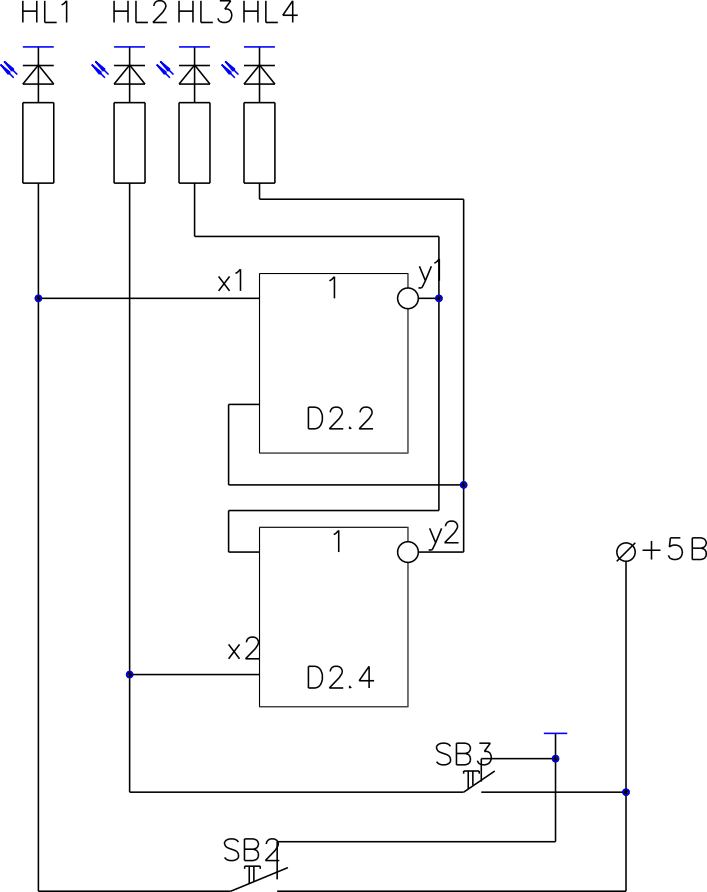
\includegraphics[width=300pt]{s1.png}
\end{figure}

% {signal: [
%   {name: 'R', wave: '0..1.0....10'},
%   {name: 'S', wave: '0.....10....'},
%   {},
%   {name: 'Q', wave: '0.....1...0.'},
%   {name: '-Q', wave: '1.....0...1.'}
% ]}


\subsection{Таблица истинности}
\begin{table}[H]
\centering
\begin{tabular}{|c|c|c|c|c|}
\hline
$SB_3 = S$ & $SB_2 = R$ & $HL_3 = Q$ & $HL_4 = \not Q$ & описание \\
\hline
1 & 0 & 1 & 0 & установка\\
0 & 0 & 1 & 0 & хранение\\
0 & 1 & 0 & 1 & сброс \\
0 & 0 & 0 & 1 & хранение \\
1 & 1 & - & - & запрещенная операция \\
\hline
\end{tabular}
\end{table}

\subsection{Временная диаграмма}
\begin{figure}[H]
    \centering
    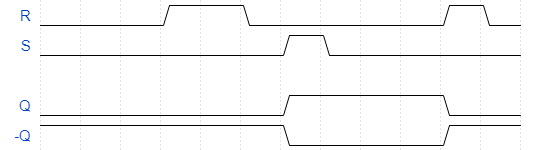
\includegraphics[width=300pt]{d1.png}
\end{figure}


\subsection{Вывод}
Асинхронный $RS$-триггер на элементах ИЛИ-НЕ.

\section{Схема II-2}

\subsection{Рисунок}
\begin{figure}[H]
    \centering
    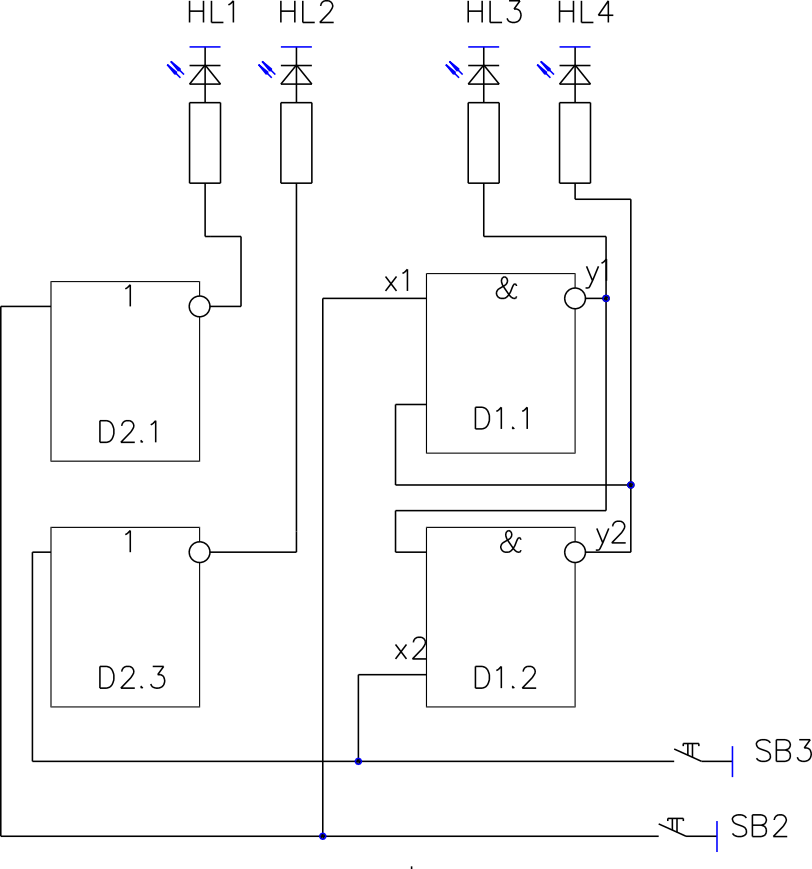
\includegraphics[width=300pt]{s2.png}
\end{figure}


% НЕПОНЯТНо ЧО ТАКОЕ R S Q .....
% {signal: [
%   {name: 'R', wave: '1..0.1....01'},
%   {name: 'S', wave: '1.....01....'},
%   {},
%   {name: 'Q', wave: '0.....1...0.'},
%   {name: '-Q', wave: '1.....0...1.'}
% ]}

\begin{table}[ht]
\centering
\begin{tabular}{|c|c|c|c|c|}
\hline
$SB_2 = S$ & $SB_3 = R$ & $HL_3 = Q$ & $HL_4 = \not Q$ & описание \\
\hline
0 & 1 & 1 & 0 & установка\\
1 & 1 & 1 & 0 & хранение\\
1 & 0 & 0 & 1 & сброс \\
1 & 1 & 0 & 1 & хранение \\
0 & 0 & - & - & запрещенная операция \\
\hline
\end{tabular}
\end{table}

\subsection{Временная диаграмма}
\begin{figure}[H]
    \centering
    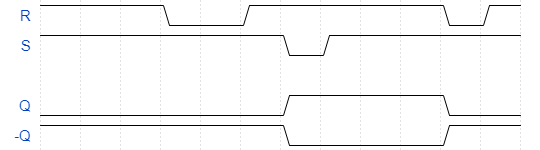
\includegraphics[width=300pt]{d2.png}
\end{figure}


\subsection{Вывод}
Асинхронный $RS$-триггер на элементах И-НЕ.

\section{Схема II-3}

\subsection{Рисунок}
\begin{figure}[H]
    \centering
    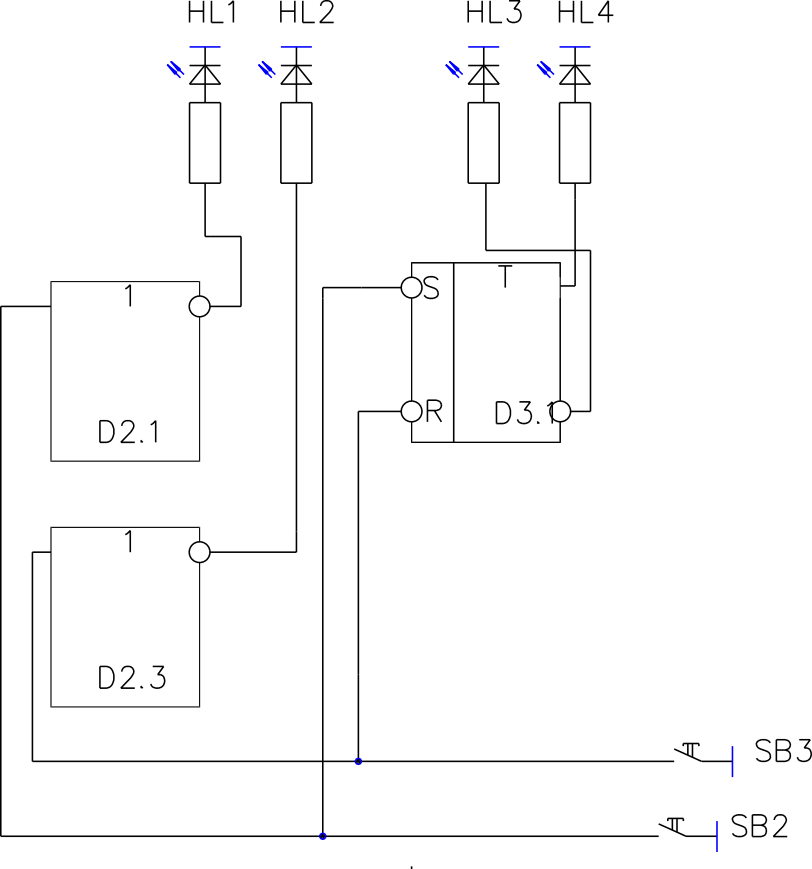
\includegraphics[width=300pt]{s3.png}
\end{figure}

\subsection{Таблица истинности}
\begin{table}[H]
\centering
\begin{tabular}{|c|c|c|c|c|}
\hline
$SB_2 = S$ & $SB_3 = R$ & $HL_4 = Q$ & $HL_3 = \not Q$ & описание \\
\hline
1 & 0 & 1 & 0 & установка\\
0 & 0 & 1 & 0 & хранение\\
0 & 1 & 0 & 1 & сброс \\
0 & 0 & 0 & 1 & хранение \\
1 & 1 & - & - & запрещенная операция \\
\hline
\end{tabular}
\end{table}

\subsection{Временная диаграмма}
\begin{figure}[H]
    \centering
    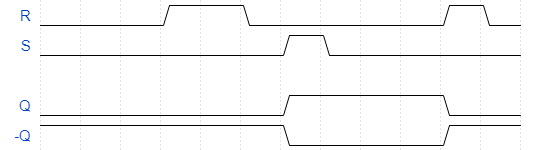
\includegraphics[width=300pt]{d1.png}
\end{figure}

\subsection{Вывод}
Асинхронный $RS$-триггер на элементах ИЛИ-НЕ.


\section{Схема II-4}

\subsection{Рисунок}
\begin{figure}[H]
    \centering
    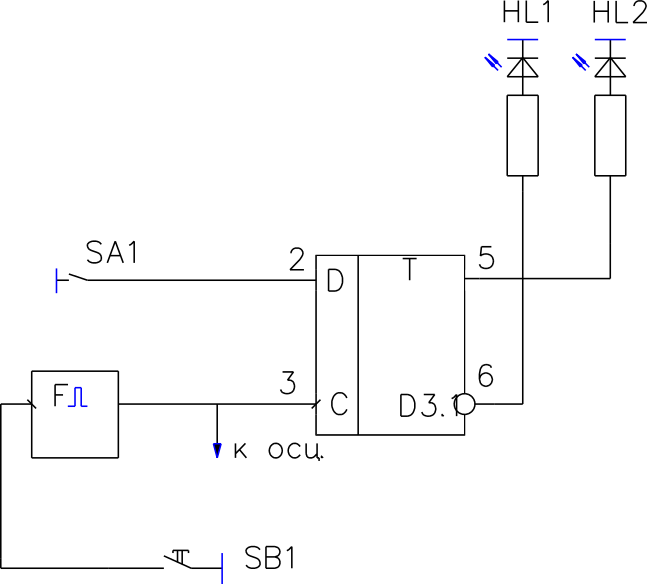
\includegraphics[width=300pt]{s4.png}
\end{figure}

% {signal: [
%   {name: 'SA1', wave: '01010101010101'},
%   {name: 'SB1', wave: '0..1..0..1..0.'},
%   {},
%   {name: 'HL2', wave: '0...1.0...1.0.'},
%   {name: 'HL1', wave: '1...0.1...0.1.'}
% ]}

\subsection{Временная диаграмма}
\begin{figure}[H]
    \centering
    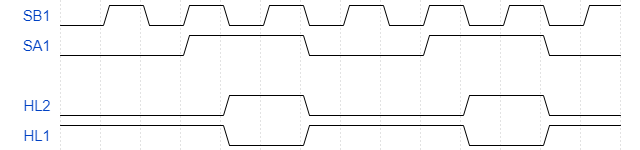
\includegraphics[width=300pt]{d4.png}
\end{figure}


\subsection{Вывод}
По спаду.



\section{Схема II-5}

% {signal: [
%   {name: 'SB1', wave: '01010101010101'},
%   {name: 'SA1', wave: '0.....1.......'},
%   {name: 'SA3', wave: '0..1..0..1....'},
%   {},
%   {name: 'HL1', wave: '0...1.0...1...'},
%   {name: 'HL2', wave: '0.....1.......'}
% ]}


\subsection{Рисунок}
\begin{figure}[H]
    \centering
    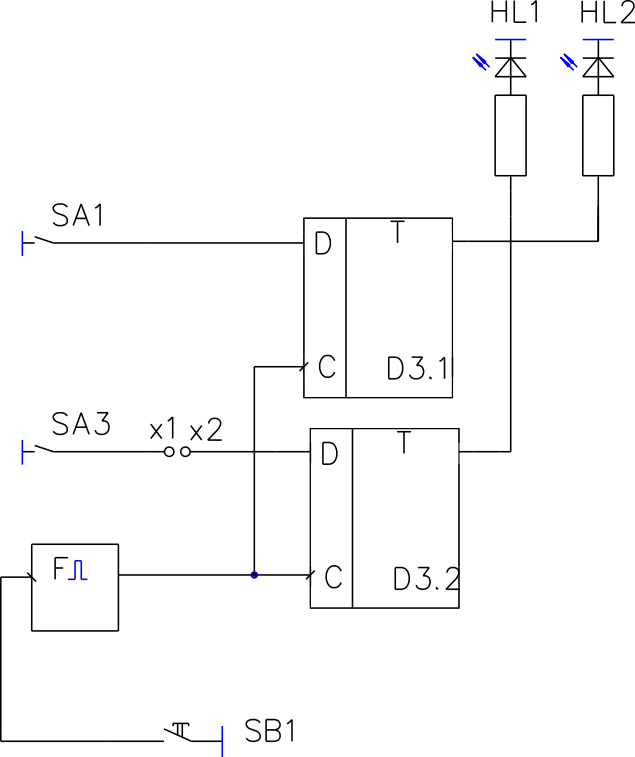
\includegraphics[width=300pt]{s5.png}
\end{figure}

\subsection{Временная диаграмма}
\begin{figure}[H]
    \centering
    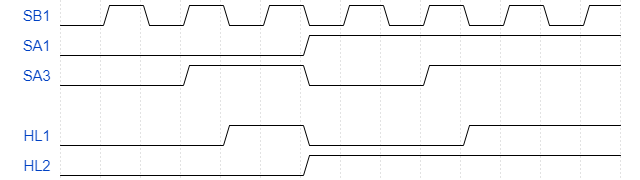
\includegraphics[width=300pt]{d5.png}
\end{figure}


\subsection{Вывод}
Параллельный регистр по спаду


\section{Схема II-6}

% {signal: [
%   {name: 'SA1', wave: '0.....1........0....'},
%   {name: 'SB1', wave: '0..10.101.01010.10.1'},
  
%   {},
%   {name: 'HL1', wave: '0......1.......0....'},
%   {name: 'HL2', wave: '0.........1.........'}
% ]}

\subsection{Рисунок}
\begin{figure}[H]
    \centering
    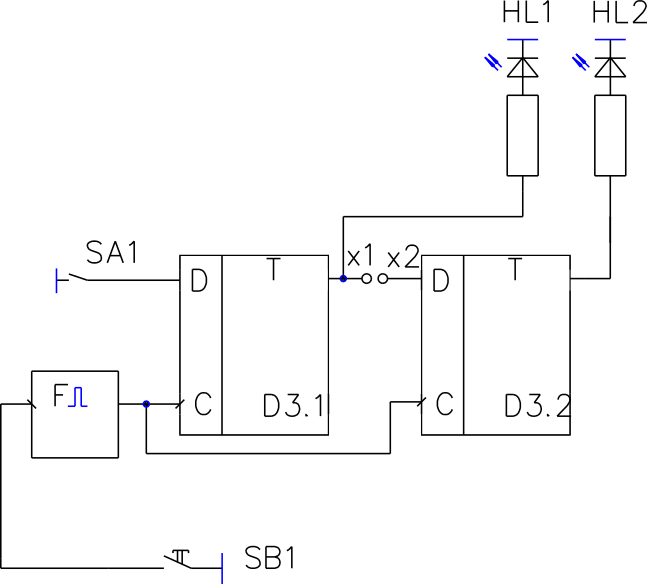
\includegraphics[width=300pt]{s6.png}
\end{figure}

\subsection{Временная диаграмма}
\begin{figure}[H]
    \centering
    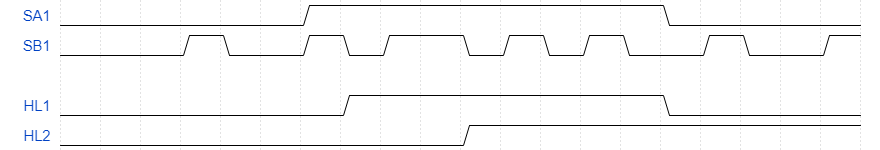
\includegraphics[width=300pt]{d6.png}
\end{figure}


\subsection{Вывод}
Последовательный регистр по спаду


\section{Схема II-7}


% {signal: [
%   {name: 'SB1', wave: '01010..1.0.1..0.10....'},
%   {},
%   {name: 'HL1', wave: '0.1.0....1....0..1....'},
% ]}


\subsection{Рисунок}
\begin{figure}[H]
    \centering
    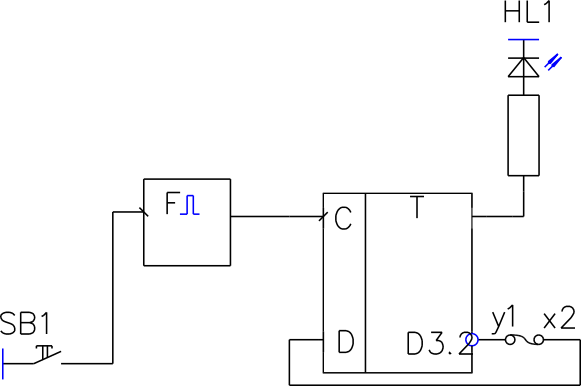
\includegraphics[width=300pt]{s7.png}
\end{figure}

\subsection{Временная диаграмма}
\begin{figure}[H]
    \centering
    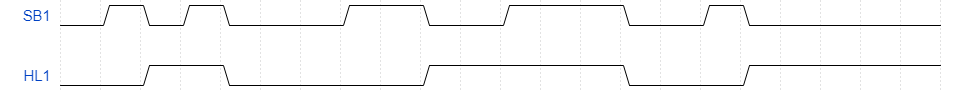
\includegraphics[width=300pt]{d7.png}
\end{figure}


\subsection{Вывод}
По спаду.

\end{document}